\documentclass[11pt]{article}
\usepackage{graphicx}
\usepackage[margin=1in]{geometry}  
\usepackage{setspace}              
\onehalfspacing         
\usepackage[T1]{fontenc}        
\usepackage[utf8]{inputenc}         
\usepackage{lmodern}           
\usepackage{amsmath, amssymb, amsthm} 
\usepackage{booktabs}    
\usepackage{array}                    
\usepackage{caption}         
\usepackage{url}         
\usepackage{hyperref} 
\usepackage{authblk}
\usepackage{rotating}
\usepackage{placeins}
\usepackage{natbib}  

\providecommand{\keywords}[1]
{
  \small	
  \textbf{\textit{Keywords---}} #1
}
\captionsetup{labelsep=period,labelfont=bf}



\title{Variance Has a Position:\\ \large{A League-Wide Signal in Box-Score Projection Error}}

\author{Nathan Humphrey\thanks{Contact: mr.nathanhumphrey@gmail.com}} \affil{Independent Researcher; Annapolis, MD\\ ORCID: 0009-0004-8512-4105}

\date{June 2026}

\begin{document}

\maketitle

\begin{abstract}
\noindent
Every projection system is evaluated on how close its forecasts land -- the mean error. We show that the variance of that error carries a structured, position-specific signal that the mean does not, and that the signal replicates across leagues and methods in a way that rules out the usual artifact explanations. After conditioning on prior-season production, position, age, and team context, the projection-error variance of blocks for centers is elevated by a factor of $1.26$ to $2.03$ relative to the rest of the league, and it couples in all $11$ testable cells across four leagues (NBA, WNBA, NCAA Division I men's and women's) under two projection methods that share no machinery. The signal is selective: center scoring runs the opposite way (centers are more predictable scorers, in all $11$ cells), veteran assists show no structure, and a center-rebounding effect that appeared under the simple method dissolves under the hierarchical one -- a retraction we report at equal prominence. We argue the block result is the measurable fingerprint of a mechanism the analytics literature has understood qualitatively since the Dwight effect \citep{goldsberry2013dwight}: a block is a noisy proxy for rim deterrence, and a proxy inherits both the variance of the skill it tracks and the variance of its own noise. We pre-register a forward test on the 2026-27 season.
\end{abstract}

\section{The signal in the error, not the estimate}\label{sec-signal}
The entire public and private apparatus of basketball projections is graded one way: a system emits a forecast, the season is played, and the system is scored on how close the forecast landed. Mean absolute error, root-mean-square error, calibration of the central estimate -- every leaderboard, every model bake-off, every "who projected the best" post-mortem lives on the distance between the point estimate and the outcome. The error's mean is the whole game.

This paper is about the error's variance, and the claim is that the variance is not uniform noise. For specific combinations of statistic and position, players miss their projections by systematically more than the rest of the league does -- not biased high or low, but more spread out -- after the obvious predictors (last season's production, position, age, team) have been conditioned away. The dispersion of the miss is itself a structured quantity, and it points at something real about which box-score numbers are trustworthy and which are not.

The loudest instance is a single cell: blocks, by centers. A center's block projection is, in a precise and replicable sense, the least trustworthy line on the stat sheet -- its error variance runs between a quarter again and twice the league baseline -- and that unreliability is not a quirk of any one model or league. It survives a change of projection method, and it reappears in the WNBA, and in men's and women's college basketball. A signal that crosses leagues that share no players and survives methods that share no machinery is not an artifact. It is a property of the thing being measured.

We make three moves. First (Section~\ref{sec-dwight}) we place the result in the lineage that explains it -- the interior-defense analytics tradition that began by showing the block is a proxy, not a skill. Second (Sections~\ref{sec-measured}--\ref{sec-selective}) we measure the signal and show it is selective -- present for blocks-by-centers, inverted for scoring, absent for veteran assists, and retracted for rebounding -- which is what separates a finding from a fishing expedition. Third (Section~\ref{sec-forward}) we commit to a forward test.

\section{The Dwight effect and the proxy problem}\label{sec-dwight}
The intellectual anchor of this paper is the most-cited result in interior-defense analytics, and we treat it as the load-bearing lineage rather than a passing reference.

\citet{goldsberry2013dwight}, in the work that named the Dwight effect, used optical tracking to show that the value of a rim protector lies in deterrence (opponents declining to attack the rim at all) rather than in the block itself. Their central demonstration was a dissociation: the league's leader in blocks was not the league's best \emph{interior} defender, because the quantity that matters is the frequency of close attempts a defender faces, not the subset of them he swats. Since roughly $70\%$ of close attempts yield points, free throws, or offensive rebounds, suppressing how often opponents even try at the rim dominates any marginal change in their efficiency. In their framing, the block is a side effect of deterrence, observed when deterrence happens to fail and the shot goes up anyway -- not the mechanism of rim protection.

\citet{franks2015counterpoints} sharpened this from descriptive into measured. Using player-tracking matchup estimates, they decomposed interior defense into a volume score (how often a defender's assignment even attempts a shot) and a disruption score (how much the defender lowers efficiency when shots do occur) and found that centers as a class derive far more of their defensive value from volume reduction than from disruption. This is the same claim as the Dwight effect, now with a coefficient on it: the deterrent who suppresses attempts is doing the work, and his block count is at best a lagging, noisy indicator of it. The broader tracking-era program around expected possession value \citep{cervone2016multiresolution} established the same lesson system-wide -- that the events the box score records are coarse summaries of a continuous process the box score cannot see.

By the present day the measurement of deterrence is mature and commoditized. Public and proprietary systems -- the Bruin Sports Analytics deterrence metric \citep{bruin2021deterrence} and the family of impact measures including Basketball Index's Help Defense and Defensive Playmaking components -- now routinely identify the defender who anchors the rim without piling up blocks. The existence of the block-shy deterrer is, by 2026, common knowledge in analytics rooms.

Here is the gap the lineage leaves open, and it is the gap this paper fills. The Dwight effect is a statement about the mean: on average, blocks understate deterrence and the leader in blocks is not the best defender. It is not a statement about variance. If a block is a noisy proxy for a latent deterrence skill, the proxy relationship has a second, untested consequence: the projection error of block counts should be anomalously large, because a center's observed blocks layer scheme, help responsibility, coaching instruction, and shot-luck noise on top of whatever stable skill they imperfectly track. Two centers with identical deterrence ability can post very different block totals, and a forecaster who projects the proxy rather than the skill should miss by an unusually wide margin. The qualitative proxy claim of 2013 predicts a variance signature in 2026 projection error -- and that signature, measured across four leagues, is the contribution of this paper. The archetype-clustering literature, which reliably recovers the rim-protecting big as a descriptive cluster \citep{cheng2017eighttypes}, is cross-sectional and silent on this; the one prior link from a big-man type to a longitudinal outcome is offensive, not defensive.

We separate this paper from its companion. The career-outcome consequence of the deterrence skill -- whether the latent quantity the blocks track predicts which centers have successful careers -- is developed elsewhere \citep{humphrey_deterrence}. The present paper is about the projection-error signature alone, and it stands whether or not the deterrence interpretation is the correct reading of why the signature exists.

\section{The variance lens, and why the mean misses it}\label{sec-lens}
The methodological frame is standard and worth stating in one paragraph, because it is what makes the result legible to a forecaster. Hierarchical and empirical Bayes projection systems -- the dominant paradigm since the Stein-shrinkage insight entered sports forecasting \citep{efron1977stein, brown2008season} -- are built to get the mean right: they shrink noisy individual estimates toward pooled group means and are evaluated on the resulting point-forecast error. What they are not built to surface is whether the residual error, after shrinkage, is itself structured by group. A class of players can be projected with a correctly centered mean and still miss with systematically larger variance than the model assumes. Since the model is scored on mean error, that excess variance is invisible to the scorecard. It lives in the residuals, which is exactly where we look.

Concretely, for each statistic and player we form a season-ahead projection, observe the realized value, and compute the standardized residual -- the miss. We then compare the variance of the residuals for a position cell against the variance for the rest of the league, conditioning on prior production, position, age, and team. The test statistic is a variance ratio, and we test its departure from $1.0$ with Levene's test \citep{levene1960}. A ratio of $1.0$ means the cell is no harder to project than the league; a ratio above $1.0$ means the cell's outcomes scatter more widely than the model expects.

\section{The signal, measured}\label{sec-measured}
The block-by-center variance ratio is consistently and substantially above $1.0$. Across all four leagues and both projection methods -- eleven testable cells in total -- every cell couples, with ratios in a band of $1.26$ to $2.03$ (Table~\ref{tbl-crossleague}, Figure~\ref{fig-forest}). The two methods are deliberately unrelated: a career-mean method that projects each player from their own weighted history, and a hierarchical negative-binomial model fit in Stan \citep{carpenter2017stan} that pools information across players. Under the career-mean method the ratios run $1.71$ to $2.03$; under the hierarchical method, $1.26$ to $1.84$. The cohort sizes span two orders of magnitude -- from 21 centers in a single NBA cross-season cell to 224 in the NCAA women's pool -- and the magnitude band holds across that range.

\begin{table}[h]
\centering
\caption{Block projection-error variance ratio (center vs.\ rest of league),
all four leagues $\times$ two methods. All 11 testable cells couple; band
1.26--2.03. NBA hierarchical cells marked (dir.) are directionally identical but
underpowered at $n = 21$ (see Table~\ref{tbl-crossseason}). Method bands:
career-mean 1.71--2.03, hierarchical 1.26--1.84.}
\label{tbl-crossleague}
\begin{tabular}{llcc}
\toprule
League & Method & Variance ratio (BLK $\times$ Center) & Couples? \\
\midrule
NBA    & career-mean         & 1.71--1.98   & yes \\
NBA    & hierarchical (Stan) & 1.24--1.26\textsuperscript{*} & yes (dir.) \\
WNBA   & career-mean         & 1.84         & yes \\
WNBA   & hierarchical        & 1.42         & yes \\
NCAA M & career-mean         & 1.79         & yes \\
NCAA M & hierarchical        & 1.55         & yes \\
NCAA W & career-mean         & 2.03         & yes \\
NCAA W & hierarchical        & 1.68         & yes \\
\bottomrule
\end{tabular}

\smallskip
{\footnotesize\textsuperscript{*}Directionally identical to the career-mean
result but short of significance at $n = 21$; see Table~\ref{tbl-crossseason}.}
\end{table}

\begin{figure}[h]
\centering
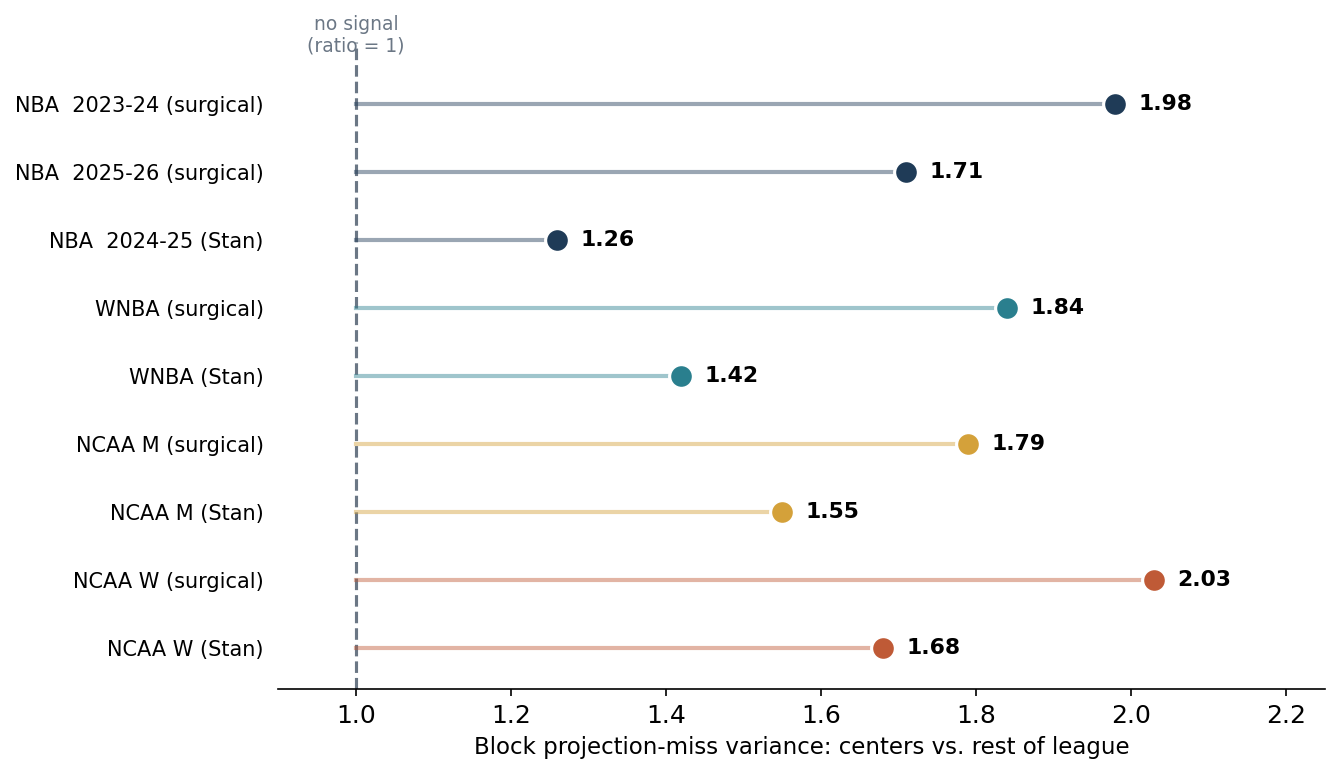
\includegraphics[width=0.85\linewidth]{figures/fig1_cross_league_forest}
\caption{Block projection-error variance ratio, centers vs.\ the rest of the
league, across four leagues and two forecasting methods. Each point is the ratio
of center error-variance to non-center error-variance; the dashed line at $1.0$
is the no-signal mark. All eleven cells sit above it, in a band of $1.26$ to
$2.03$. Colors group leagues.}
\label{fig-forest}
\end{figure}

Two features defeat the standard artifact explanations. First, the signal replicates across leagues that share no players and no scorekeepers: a quirk of NBA officiating or one data provider's block definition cannot reproduce the same elevated ratio in the WNBA and in men's and women's college basketball. Second, it replicates across two methods that share no machinery: if the excess variance were an artifact of how one model shrinks, a structurally different model would not reproduce it. It does. Table~\ref{tbl-crossseason} gives the within-NBA cross-season detail, where the cohort is cleanest and the significance is strongest -- the 2025--26 cell reaches Levene $p=4.7 \times 10^{-8}$ at $n=71$ centers, while the underpowered 2024--25 cell ($n=21$) is directionally identical but short of significance, a power limitation rather than a contradiction.

\begin{table}[h]
\centering
\caption{Block projection-error variance for centers vs.\ the rest of the
league, NBA, three consecutive seasons (hierarchical method). The 2025-26 cell,
with the largest center sample, is significant beyond one in ten million; the
2024-25 cell ($n = 21$) is directionally identical but underpowered.}
\label{tbl-crossseason}
\begin{tabular}{lcccccc}
\toprule
Season & Centers ($n$) & Rest ($n$) & Center miss-SD & Rest miss-SD & Ratio & Levene $p$ \\
\midrule
2023-24 & 21 & 132 & 0.371 & 0.187 & 1.98 & $0.002$ \\
2024-25 & 21 & 110 & 0.236 & 0.189 & 1.24 & $0.112$ \\
2025-26 & 71 & 414 & 0.368 & 0.215 & 1.71 & $4.7 \times 10^{-8}$ \\
\bottomrule
\end{tabular}
\end{table}

The translation for anyone who builds or reads a projection is direct: a center's block number is the single least reliable line on the sheet, and the unreliability is structural, not seasonal. A center projected for $1.5$ blocks is genuinely more likely to finish at $0.8$ or $2.3$ than a guard projected for $1.5$ assists is to land equally far from his mark. The spread is the information.

\section{The signal is selective}\label{sec-selective}
A signal that appeared in every cell would indicate a fishing expedition or a global miscalibration, not a finding. The block result earns its credibility because the same machinery, pointed at three other stat-and-position cells, returns three different verdicts -- including a retraction (Figure~\ref{fig-verdicts}).

\subsection{Points by centers run the other way}
Applied to scoring, the identical comparison returns a variance ratio below $1.0$ -- centers are more predictable scorers than the rest of the league -- in all $11$ testable cells. The direction is consistent everywhere; it reaches formal significance only at the large NCAA cohort sizes, where 3 of 4 hierarchical cells clear Levene's test (the fourth at $p=0.056$), because the professional cohorts ($n=21$ to $71$) are too small to detect a small effect. This is the mirror image of the block result and it makes basketball sense: a center's scoring comes from high-percentage looks near the rim and from a role the offense defines, so it is anchored in a way his block totals are not.

\subsection{Veteran assists show nothing}
The assists of long-tenured veterans return a variance ratio at $1.0$ -- a clean process-only null, replicated in $6$ of $6$ cells across NBA cross-season tests and the WNBA. There is no hidden structure in that cell; it is the null against which the others are measured, and it confirms the method does not manufacture signal where none exists.

\subsection{Rebounds by centers looked real and were not}
Under the career-mean method, center rebounding showed an elevated variance ratio that resembled the block signal. Under the hierarchical method it vanished, in every league where the robustness check was run ($0$ of $7$ cells). The diagnosis is clean: the apparent signal was position-level mean structure that the hierarchical model correctly absorbs into its center mean, leaving no residual-variance asymmetry. The four-league rebounding pattern is a position-mean finding, not a projection-error-variance finding, and we were wrong to read it as the latter in an earlier cut. We report the walk-back at the same volume as the confirmations, because a paper that reported only its hits would not deserve trust on the block result. This is the cell that earns it.

Read together, the four verdicts are the argument. Blocks scatter more than expected; scoring less; veteran assists exactly as expected; rebounding looked structured until a better model showed it was mean structure in disguise. A fishing expedition finds signal everywhere. This finds it in one place, finds its inverse in a second, finds nothing in a third, and recants a fourth -- which is the signature of a real effect, not an artifact of the search.

\begin{figure}[h]
\centering
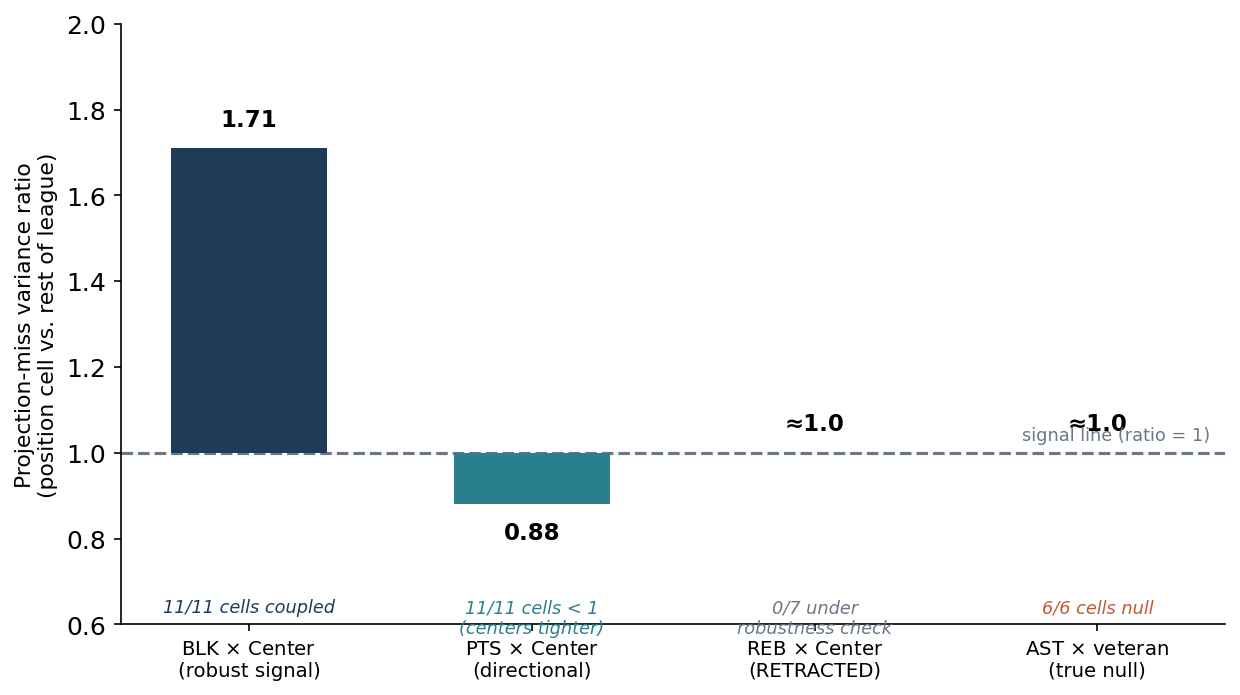
\includegraphics[width=0.9\linewidth]{figures/fig2_four_verdicts}
\caption{Four stat-and-position cells, four verdicts. Blocks by centers carry
elevated error-variance (robust signal, 11/11 cells). Points by centers run the
other way -- centers are \emph{more} predictable scorers (directional, 11/11
cells below $1.0$). Rebounds by centers looked elevated under the career-mean
method but dissolved under the hierarchical one (retracted, 0/7). Veteran
assists show no structure (true null, 6/6). The dashed line is the no-signal
mark.}
\label{fig-verdicts}
\end{figure}

\section{What it means on the floor, and one methodological consequence}\label{sec-cons}
If a center's block total is the least reliable number on his sheet, three things follow for evaluation. Blocks are the worst single statistic to anchor a center's defensive grade on -- not because they are meaningless, but because their year-to-year scatter is so wide that any one season's total is a weak read on the underlying skill; a drop from $2.4$ to $1.1$ blocks may be entirely inside the normal range and signal no decline at all. The stability of the number is itself a scouting variable: a center whose block totals swing wildly across seasons and schemes is more likely a scheme-dependent rim protector than one whose deterrence is portable. And the cells that are tight (center scoring, veteran assists) are the projections that mean what they say.

There is also a methodological consequence that matters to anyone running a Bayesian projection system. The variance signal is invisible to a system scored on mean error, which means production systems routinely ship miscalibrated intervals on exactly these cells -- a $50\%$ predicted interval on center blocks can empirically cover far less than $50\%$ of outcomes, because the model's predicted interval reflects only the variance its count process assumes, while the realized outcomes carry the additional position-specific dispersion this paper documents. The variance lens is, among other things, a calibration diagnostic: it flags the cells where a system's stated confidence is most overrated.

\section{Scope and a forward test}\label{sec-forward}
The result is a statement about predictability, measured on projection systems -- it says block totals are hard to forecast for centers, not that blocks are "wrong.'' Its strength is replication: the same elevated ratio in four leagues under two unrelated methods is very hard to produce by accident. The main constraint is professional cohort size -- NBA and WNBA center cells run as small as $21$ players, which is why effects that are clearly present in direction (center scoring's lower variance) reach formal significance only at NCAA scale. Where the professional cells fall short, they fall short on power, not direction.

The cleanest test is one fixed before the data exist. We pre-register, before the 2026--27 season generates any results: the block projection-error variance for centers will again exceed the rest-of-league variance, with a ratio in the $1.26$-to-$2.03$ band, under the same conditioning and the same two methods used here; and the center-scoring cell will again show a ratio below $1.0$. A center-block ratio at or below $1.0$, or a reversal of the scoring direction, falsifies the corresponding claim. The registration is timestamped before the season opener.

\bibliographystyle{apalike}
\bibliography{references}

\end{document}
